\documentclass[11pt]{article}
\newcommand\comment[1]{}
\usepackage{graphicx}
\usepackage{a4wide,parskip,times}


\newcommand{\todo}[1]{\textbf{#1}}
\newcommand{\deno}[1]{{\bf [\![}#1{\bf ]\!]}}



\newcommand{\st}{$^{st}$}
\renewcommand{\th}{$^{th}$}
\newcommand{\nd}{$^{nd}$}
\newcommand{\rd}{$^{rd}$}

\begin{document}

\centerline{\Large Multicore Semantics and Programming}
\vspace{2em}
\centerline{\Large \emph{Pratical Report}}
\vspace{2em}
\centerline{\large A. J. Taylor (\emph{at736}), St John's College}
\vspace{1em}

\begin{abstract}
\textsl{
	A written report for Tim Harris' section of the course
} 
\end{abstract}


\section{Summary of Experimental Conditions and Methods}

\subsection{Hardware}
Experiments were carried out on a HP Spectre Laptop, which was plugged in and on maximum performance settings. 

The laptop has a quad core, hyperthreaded, intel i7 8550u processor for a total of 8 physical threads (two threads per core) \footnote{https://ark.intel.com/products/122589/Intel-Core-i7-8550U-Processor-8M-Cache-up-to-4-00-GHz-}.

\subsection{Experimental Methods}
Experiments were written in Java and run under Windows 10. The laptop was set not to sleep for the duration of each experiment and other user processes were kept to a minimum to improve reliability of the results.

\subsection{Code Written}
The code used to run experiments and process the resulting data can be found on a dedicated Github repository\footnote{https://github.com/Al153/MulticoreSemantics}. I created an abstract \texttt{SharedArray} class containing an array with specifiable length and an abstract \texttt{sum} (read) and \texttt{update} (write) operations. Appropriate subclasses of this class were created with the \texttt{sum} and \texttt{update} operations taking the correct locks.


\section{The Experiments}
\subsection{Set Up and Initial Test}
The supplied test code ran correctly.
\subsection{Simple Multithreading}
\begin{figure}\label{step2_1}
\centering
\includegraphics[scale=0.65]{step2.png}
 \caption{Time to complete for each thread running. Error bars, as is the case in the rest of this report, represent a single standard deviation on either side.}
\end{figure}

In this experiment, repeated 100 times per number of threads, performance stays roughly equal for $n = 1, 2$, then begins to increase monotonically. As might be expected, there is a larger increase between $n= 4k$ and $n= 4k +1$.

\todo{Explanation}


\subsection{Read Only Shared-Arrays}
\paragraph{Unsafe Shared Array}

\begin{figure}\label{step3_1}
\centering
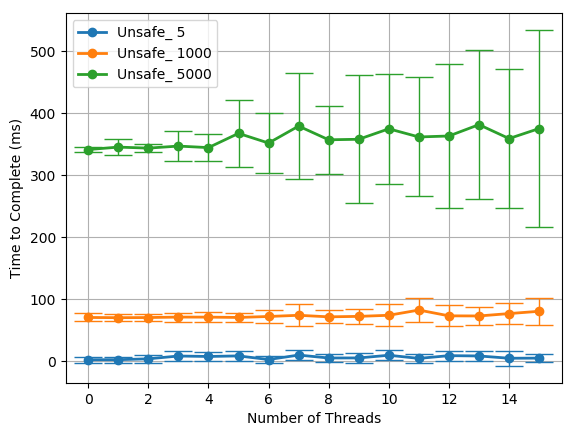
\includegraphics[scale=0.65]{step3_1.png}
\caption{Speed of the unsafe shared array when instantiated with various sizes}
\end{figure}


\begin{figure}\label{step3_2}
\centering
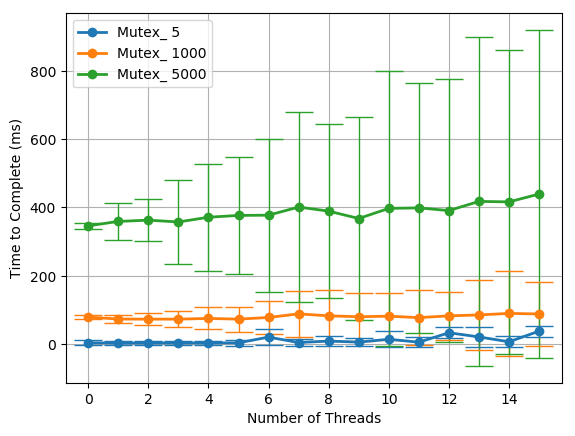
\includegraphics[scale=0.65]{step3_2.png}
\caption{Speed of the safe, mutex locked, shared array when instantiated with various sizes}
\end{figure}

The locked array did not perform significantly worse in the average case than the unsafe array,
however the variance increases significantly as the number of threads and size of the array increases. I expect this is due to a one sided distribution, where the majority of results are scattered close to the mean with some large outliers which took much longer due to a delay in loading and taking a lock.

\todo{explanation}


\begin{figure}\label{step3_3}
\centering
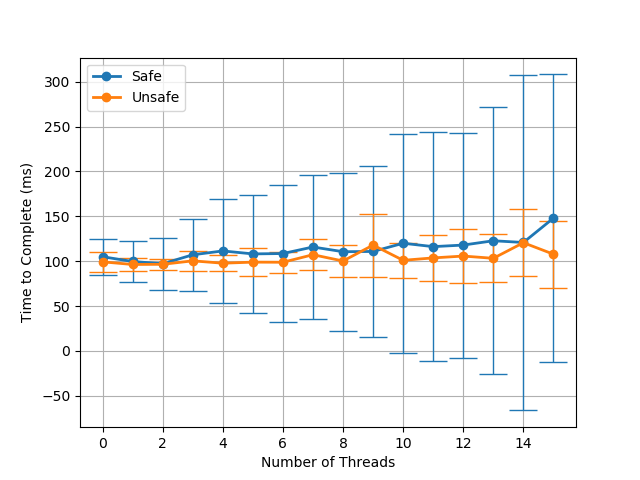
\includegraphics[scale=0.65]{step3_3.png}
\caption{Comparative speed of the unsafe and mutex-locked arrays set to a size of $X=5000$. The standard deviation is much more constant for the unsafe version.}
\end{figure}


\subsection{TATAS Lock}

\begin{figure}\label{step4_1}
\centering
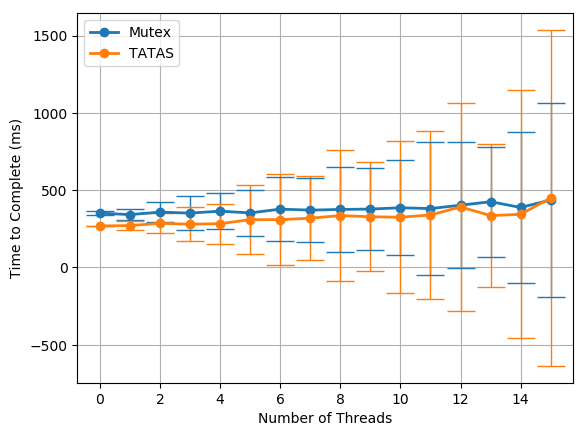
\includegraphics[scale=0.65]{step4_1.png}
\caption{Speed of the mutex-locked and TaTaS shared arrays for $X=5000$}
\end{figure}


The TaTaS-lock performed slightly better than the mutex-lock for small numbers of threads due to its better cache line behaviour, but as the number increased, the performance of the TaTaS lock deteriorated and the standard deviation of its operation increased greatly.

\subsection{Reader-Writer Lock}
\begin{figure}\label{step5_1}
\centering
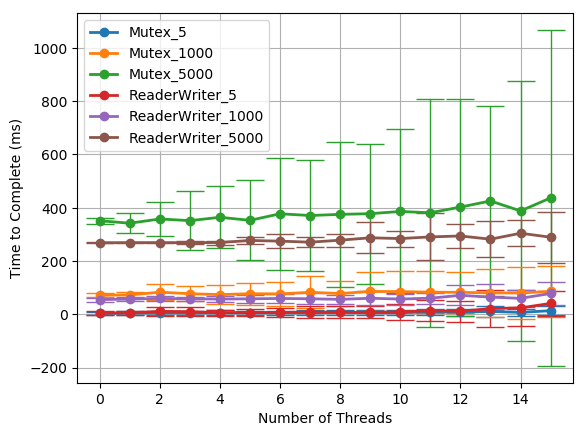
\includegraphics[scale=0.65]{step5_1.png}
\caption{Speed of the mutex-locked array versus the reader-writer locked array when instantiated with various sizes}
\end{figure}

\subsection{Reader-Writer Lock}
\begin{figure}\label{step5_2}
\centering
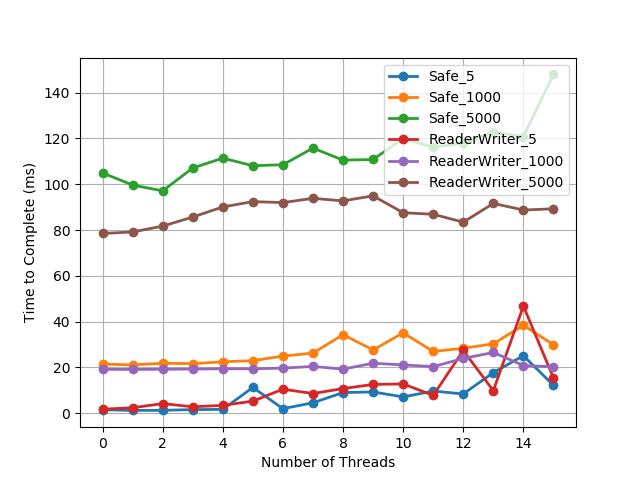
\includegraphics[scale=0.65]{step5_2.png}
\caption{Speed of the mutex-locked array versus the reader-writer locked array when instantiated with various sizes, drawn without error bars to more clearly show the mean-behaviour.}
\end{figure}

When the array size is not negligibly small, the reader-writer lock significantly outperforms the standard mutex lock as it allows multiple summing operations to occur at once.

\subsection{Flag-Based Lock}

\subsection{Reader-Writer Lock}
\begin{figure}\label{step6_1}
\centering
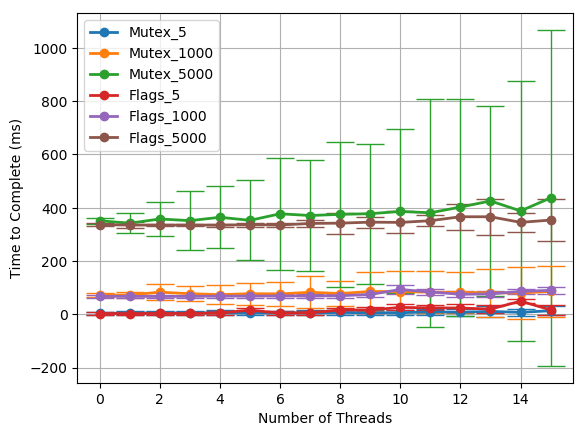
\includegraphics[scale=0.65]{step6_1.png}
\caption{Speed of the mutex-locked array versus the flag-locked array when instantiated with various sizes}
\end{figure}

The flag based lock outperformed the mutex-lock less significantly than the reader-writer lock but with a tighter standard deviation. \todo{clearer}

\subsection{Reader-Writer Lock}
\begin{figure}\label{step6_2}
\centering
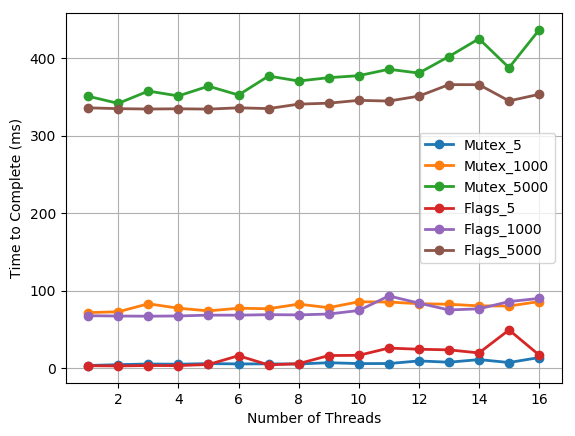
\includegraphics[scale=0.65]{step6_2.png}
\caption{Speed of the mutex-locked array versus the flag-locked array when instantiated with various sizes, drawn without error bars to more clearly show the mean-behaviour.}
\end{figure}

\subsection{Write Mode}

\begin{figure}\label{step7_1}
\centering
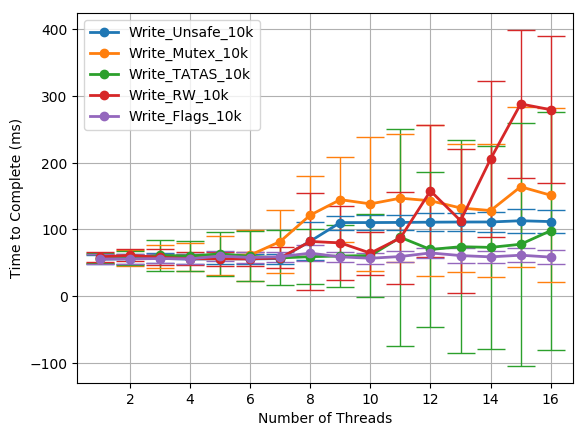
\includegraphics[scale=0.65]{step7_1.png}
\caption{Speed of the mutex-locked array versus the flag-locked array when instantiated with various sizes, drawn without error bars to more clearly show the mean-behaviour.}
\end{figure}

\begin{figure}\label{step7_2}
\centering
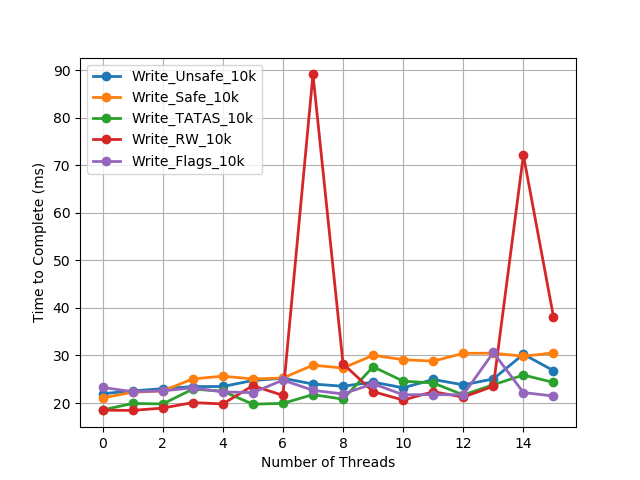
\includegraphics[scale=0.65]{step7_2.png}
\caption{Speed of the mutex-locked array versus the flag-locked array when instantiated with various sizes, drawn without error bars to more clearly show the mean-behaviour.}
\end{figure}

\begin{figure}\label{step7_3}
\centering
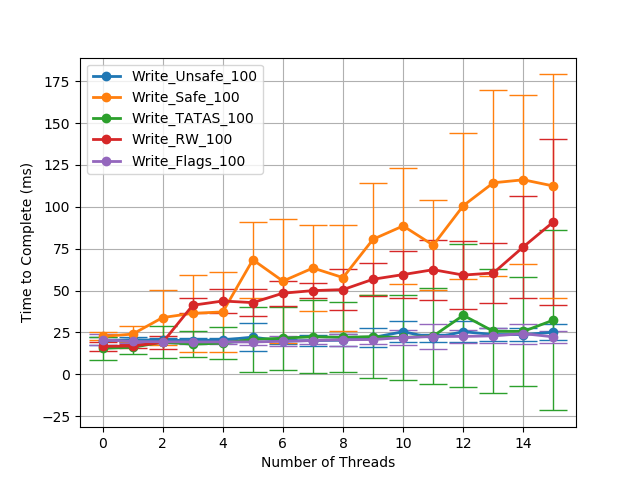
\includegraphics[scale=0.65]{step7_3.png}
\caption{Speed of the mutex-locked array versus the flag-locked array when instantiated with various sizes, drawn without error bars to more clearly show the mean-behaviour.}
\end{figure}

\begin{figure}\label{step7_4}
\centering
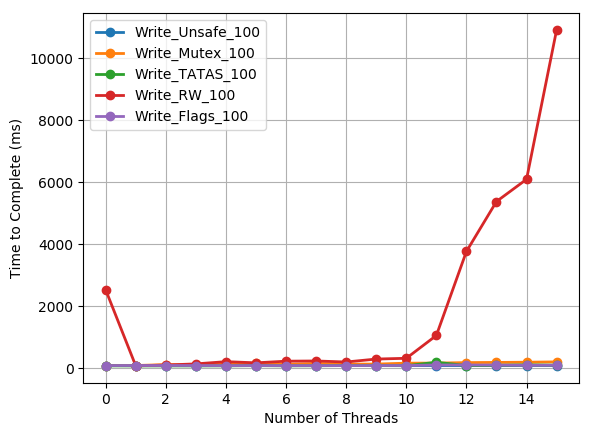
\includegraphics[scale=0.65]{step7_4.png}
\caption{Speed of the mutex-locked array versus the flag-locked array when instantiated with various sizes, drawn without error bars to more clearly show the mean-behaviour.}
\end{figure}




\section{Summary}

\end{document}